% Lima Angka dalam Satu Kotak: Diagram Kotak-Garis (Box Plot) dengan TikZ
% Dokumen LaTeX utuh, siap dikompilasi (butuh paket tikz).
% Data: 32 nilai ulangan harian Matematika kelas 8C, terurut dari kecil ke besar.
% 45, 48, 52, 55, 57, 59, 61, 63, 65, 66, 67, 68, 69, 70, 71, 73,
% 74, 75, 76, 77, 78, 79, 80, 82, 84, 85, 86, 88, 89, 91, 94, 98
% Terendah = 45 | Q1 = 64 | Median (Q2) = 73,5 | Q3 = 83 | Tertinggi = 98
% IQR = 19 ; tidak ada pencilan (pagar bawah 35,5 ; pagar atas 111,5)
\documentclass{article}
\usepackage{tikz}

\begin{document}

\section*{Diagram kotak-garis (box plot) nilai kelas 8C}

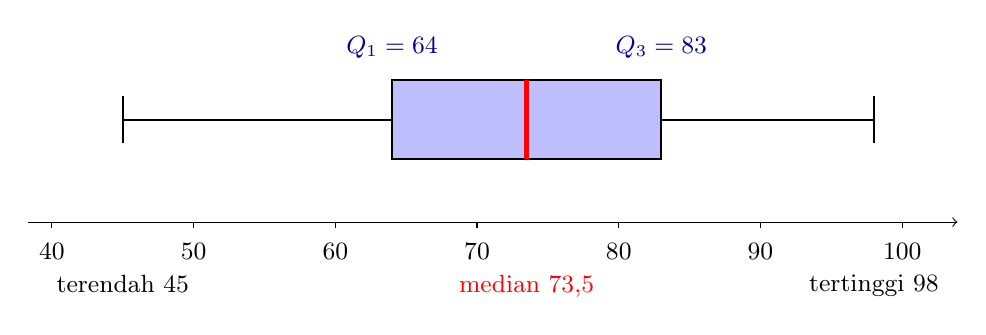
\begin{tikzpicture}
  % skala sumbu x: 0,18 cm untuk tiap 1 nilai (nilai 40 -> x=0 ; nilai 100 -> x=10,8)
  % sumbu bilangan digambar di y=0, kotak digambar di sekitar y=1,3
  \draw[->] (-0.3,0) -- (11.5,0);
  % tanda nilai pada sumbu x
  \foreach \v in {40,50,60,70,80,90,100}
    { \pgfmathsetmacro{\x}{(\v-40)*0.18}
      \draw (\x,0) -- (\x,-0.08);
      \node[below, font=\small] at (\x,-0.15) {\v}; }
  % kumis: dari nilai terendah ke Q1, dan dari Q3 ke nilai tertinggi
  % x dihitung: (nilai-40)*0,18 ; 45 -> 0,90 ; 64 -> 4,32 ; 83 -> 7,74 ; 98 -> 10,44
  \draw[thick] (0.9,1.3) -- (4.32,1.3);     % kumis kiri: 45 s.d. Q1
  \draw[thick] (7.74,1.3) -- (10.44,1.3);   % kumis kanan: Q3 s.d. 98
  \draw[thick] (0.9,1.0) -- (0.9,1.6);      % tutup kumis kiri
  \draw[thick] (10.44,1.0) -- (10.44,1.6);  % tutup kumis kanan
  % kotak: separuh tengah data (Q1=64 s.d. Q3=83)
  \draw[thick, fill=blue!25] (4.32,0.8) rectangle (7.74,1.8);
  % garis median: 73,5 -> x = (73,5-40)*0,18 = 6,03
  \draw[ultra thick, red] (6.03,0.8) -- (6.03,1.8);
  % label kelima angka, disusun bertingkat agar tidak bertumpuk
  \node[below, font=\small] at (0.9,-0.55) {terendah 45};
  \node[above, font=\small, blue!60!black] at (4.32,1.95) {$Q_1 = 64$};
  \node[below, font=\small, red] at (6.03,-0.55) {median $73{,}5$};
  \node[above, font=\small, blue!60!black] at (7.74,1.95) {$Q_3 = 83$};
  \node[below, font=\small] at (10.44,-0.55) {tertinggi 98};
\end{tikzpicture}

\end{document}
